\documentclass[10pt]{article}

\usepackage[margin=0.75in]{geometry}
\usepackage{amsmath,amssymb}
\usepackage{booktabs}
\usepackage{graphicx}
\usepackage{hyperref}
\usepackage{xcolor}
\usepackage{microtype}
\usepackage{enumitem}
\usepackage{caption}
\usepackage{multicol}
\captionsetup{font=small,labelfont=bf,skip=4pt}

\setlength{\parskip}{2pt}
\setlength{\textfloatsep}{6pt plus 1pt minus 2pt}
\setlength{\intextsep}{6pt plus 1pt minus 2pt}
\setlength{\abovedisplayskip}{4pt plus 1pt}
\setlength{\belowdisplayskip}{4pt plus 1pt}

\hypersetup{colorlinks=true, linkcolor=blue!50!black, citecolor=blue!50!black, urlcolor=blue!50!black}

\graphicspath{{figures/voronoi_p0/}{figures/}}

\newcommand{\R}{\mathbb{R}}
\newcommand{\uh}{\mathbf{u}_h}
\newcommand{\uvec}{\mathbf{u}}
\newcommand{\nv}{\mathbf{n}}
\newcommand{\xv}{\mathbf{x}}

\title{\vspace{-1.6em}Mimetic Conservative Edge-Flux Remap for Polygons}
\author{Vijay Mahadevan}
\date{\vspace{-0.6em}2026-05-05\vspace{-1em}}

\begin{document}
\maketitle

\noindent\textbf{Abstract.}\,
We present a first-order mimetic conservative method for transferring edge-normal flux degrees of freedom between two nonmatching polygonal meshes of the same domain (unit square). The method uses a two-stage pipelined approach: (i) a per-cell velocity reconstruction from edge fluxes followed by clipped-overlap edge-to-edge transfer that is exactly conservative on every source-target cell overlap; and (ii) a small constrained least-squares H(div)-conforming projection that further enforces per-target-cell discrete-divergence consistency. The output is a single signed scalar per unique target edge in the intrinsic-normal sign convention. The projected fluxes preserve global integral conservation and per-overlap conservation to machine precision, exhibit machine-precision per-target-cell discrete-divergence consistency, and converge at first order in the $L^2$ norm of edge fluxes for smooth analytical fields. Further studies are needed to combine the local Gnomonic projection with this edge-remap scheme to verify convergence for MPAS meshes on the sphere.

\smallskip
\noindent\textbf{Scope note.}\,
This report is a compact standalone reference for the lowest-order planar P0
workflow and SCRIP-style edge-weight output.  The canonical manuscript for the
current C++ codebase, including spherical, high-order, VEM, patch-recovery, and
round-trip studies, is \texttt{mimetic\_voronoi\_report.tex}.

%==========================================================
\section{Methodology}
%\subsection{Edge-flux degrees of freedom}
%==========================================================

Let $\Omega = [0,1]^2$ be tessellated into convex polygonal cells. For each unique edge $e$ with endpoints $(v_{\text{lo}}, v_{\text{hi}})$ ordered lexicographically, define the edge tangent $\mathbf{t}_e = (v_{\text{hi}} - v_{\text{lo}})/|e|$ and the intrinsic outward normal $\nv_e$ as the right-rotation of $\mathbf{t}_e$. The single primary degree of freedom on $e$ is the normal flux
\begin{equation}
\Phi_e \;:=\; \int_{e} \uvec\cdot\nv_e\,ds.
\label{eq:dof}
\end{equation}
For each cell $K$ touching $e$ a sign $\sigma_K(e)\in\{\pm 1\}$ records whether $K$'s counter-clockwise traversal of its boundary visits $e$ as $v_{\text{lo}}\!\to\!v_{\text{hi}}$ ($\sigma_K(e)=+1$) or as $v_{\text{hi}}\!\to\!v_{\text{lo}}$ ($\sigma_K(e)=-1$); the cell's outward flux on $e$ is then $\sigma_K(e)\,\Phi_e$. This signed convention is the standard choice in mixed finite element \cite{RaviartThomas1977,BrezziFortin1991} and mimetic \cite{BochevHyman2006,LipnikovManziniShashkov2014} discretisations of the H(div) space. Applying the divergence theorem to a single cell yields the discrete identity
\begin{equation}
d_K \;:=\; \frac{1}{|K|}\sum_{e\subset\partial K} \sigma_K(e)\,\Phi_e
       \;=\; \frac{1}{|K|}\!\int_K \nabla\!\cdot\!\uvec\,dA,
\label{eq:discdiv}
\end{equation}
exact whenever the edge fluxes are integrated to machine precision. Equation~\eqref{eq:discdiv} is the only mechanism by which the discrete operators carry conservation.

%==========================================================
\subsection{Local velocity reconstruction}
%==========================================================

For each source cell $K$ with $N$ edges and signed local fluxes $\{U_e\}$, the lowest-order (``level-2'') mimetic method \cite{PerotChartrand2021} reconstructs a velocity field
\begin{equation}
\uh(\xv) \;=\; \tfrac{d}{2}\,\xv \;+\; \sum_{k=1}^{K_{\max}}\!\bigl[\,a_k\,\nabla P_k(\xv) + b_k\,\nabla Q_k(\xv)\,\bigr],\quad K_{\max} = \lfloor N/2\rfloor,
\label{eq:reconform}
\end{equation}
where $P_k(x,y) + i\,Q_k(x,y) = (x+iy)^k$ in coordinates centered at the cell centroid, $\xv$ is the local position, and $d$ is the cell-mean divergence. The term $\tfrac{d}{2}\xv$ carries the full divergence ($\nabla\!\cdot\!(\tfrac{d}{2}\xv) = d$); the harmonic-gradient terms are curl-free and divergence-free, and contribute only to the rotational and irrotational parts of the field. Hence $d$ is fixed in closed form by~\eqref{eq:discdiv}: $d = (\sum_e U_e)/|K|$.

The harmonic coefficients $\{a_k, b_k\}$ are determined as the unique minimiser of the Dirichlet energy
$\tfrac12\!\int_K |\nabla\uh|^2 dA - (\text{moment forcing})$
subject to the $N{-}1$ remaining edge-flux constraints (one is automatically satisfied by~\eqref{eq:discdiv}); this is a small linear saddle-point system per cell, of size at most $(N_h + N{-}1)$ with $N_h = 2K_{\max}$. The decomposition mirrors the polynomial-divergence plus harmonic-completion split common to mixed virtual element and mixed mimetic families \cite{BrezziFalkMarini2014,BeiraoDaVeigaMixed2016}.

%\paragraph{Length scaling.}\!
Note that even though the continuous problem is well-posed, the discrete coefficient matrix's diagonal scales as $|K|^k$ for the $k$-th harmonic mode, which on refined Voronoi meshes ($h\!\sim\!10^{-2}$, $K_{\max}\!\le\!4$) drives the condition number above $10^{10}$. To overcome the ill-conditioning in such cases, the harmonic basis is evaluated in coordinates rescaled by the cell length scale $s = \max(\sqrt{|K|},\max_v|v - \mathbf{c}_K|)$ similar to approaches in \cite{LipnikovManziniShashkov2014}. This makes the system entries $\mathcal{O}(1)$ at any mesh resolution and stabilizes the coefficient recovery.

%==========================================================
\subsection{Edge-to-edge transfer with H(div)-conforming projection}
%==========================================================

The remap operator acts on the global vector of source edge fluxes and produces target edge fluxes in two stages.

\paragraph{Stage 1: Clipped-overlap assembly.}
For each target edge $e_t$ with intrinsic normal $\nv_{e_t}$:
\begin{enumerate}[label={(\roman*)},itemsep=1pt,topsep=2pt,leftmargin=*]
\item Identify candidate source cells via a spatial index on cell centroids.
\item Clip the segment $e_t$ against each candidate convex cell $K_s$ using Sutherland--Hodgman half-plane clipping \cite{SutherlandHodgman1974}, yielding a sub-segment $\subseteq e_t \cap K_s$.
\item Disambiguate sub-segments lying on a shared source-cell boundary by a perpendicular tie-breaking probe, otherwise both adjacent source cells claim the segment and the contribution is double-counted.
\item Integrate $\uh^{K_s}\!\cdot\!\nv_{e_t}$ along the sub-segment using 4-point Gauss--Legendre, expressed as a linear combination of the source cell's coefficients $(d_s, a_k, b_k)$ from~\eqref{eq:reconform}.
\item Compose with the per-cell linear coefficient map and accumulate signed contributions into the row of the assembly matrix $W$ for $e_t$.
\end{enumerate}
By construction, $W$ satisfies the constant-divergence overlap identity: summing its contributions on any source-target overlap $O = K_s \cap K_t$ gives exactly $d_s\,|O|$. This is the discrete divergence theorem applied to the constant-divergence reconstruction $\uh^{K_s}$ over $O$, and it is the lowest-order analogue of the consistency relations underlying conservative remap projection schemes \cite{Jones1999}.

\paragraph{Stage 2: H(div)-conforming projection.}
Stage 1 alone does not enforce per-target-cell discrete-divergence consistency: target cells crossing several source cells inherit the source-supported piecewise-constant divergence rather than their own cell-mean. We project $\boldsymbol\Phi^{(1)} = W\boldsymbol\Phi^{\mathrm{src}}$ onto the H(div)-conforming subspace \cite{ArnoldFalkWinther2006,BeiraoDaVeigaMixed2016} by finding the unique $\boldsymbol\Phi$ that minimises $\|\boldsymbol\Phi - \boldsymbol\Phi^{(1)}\|^2$ subject to
\begin{equation}
\sum_{e \subset \partial K_t}\!\sigma_{K_t}(e)\,\Phi_e \;=\; \sum_{K_s} d_s\,|K_s\!\cap\!K_t|
\quad\text{for every target cell }K_t,
\label{eq:hdiv-constraint}
\end{equation}
the area-weighted source-determined divergence integral on $K_t$. With $A$ the signed cell-edge incidence and $\mathbf{b}$ the right-hand side of \eqref{eq:hdiv-constraint}, the closed-form solution is $\boldsymbol\Phi = \boldsymbol\Phi^{(1)} - A^{\!\top}\!\boldsymbol\lambda$ with $A A^{\!\top}\boldsymbol\lambda = A\boldsymbol\Phi^{(1)} - \mathbf{b}$ (small sparse symmetric system, factored once per mesh pair). The output is a single signed scalar per unique target edge in the intrinsic-normal convention. The composite operator from source fluxes to projected target fluxes is what we hereafter call ``the remap'' and what the SCRIP file stores.

%==========================================================
\section{Numerical results}
%==========================================================

\noindent\textbf{Setup.}\,
Source seeds are Halton points in $(0,1)^2$ with bases $(2,3)$; target seeds use a different Halton offset and $N_t \approx 1.5\,N_s$ to guarantee fully nonmatching meshes. Both meshes use a four-mirror trick (mirror copies of every interior seed across each boundary side) to generate Voronoi tessellations exactly contained in $[0,1]^2$. Two analytical fields are studied:
\begin{align*}
\textbf{div-free:}\quad & \uvec^{\mathrm{df}}(x,y) = \bigl(\sin\!\pi x \cos\!\pi y,\ -\!\cos\!\pi x \sin\!\pi y\bigr),
& \nabla\!\cdot\!\uvec^{\mathrm{df}} \equiv 0,\\[1pt]
\textbf{smooth-div:}\quad & \uvec^{\mathrm{sd}}(x,y) = \bigl(\sin\!\pi x,\ \sin\!\pi y\bigr),
& \nabla\!\cdot\!\uvec^{\mathrm{sd}} = \pi(\cos\!\pi x + \cos\!\pi y).
\end{align*}
Note that the polynomial reconstruction~\eqref{eq:reconform} of degree $\le K_{\max}$ on each cell exactly recovers only constants on arbitrary Voronoi cells. The transcendental fields above lie outside the per-cell polynomial space, so the edge-flux error converges as $\mathcal{O}(h)$ rather than vanishing identically (this is true regardless of whether the field is divergence-free).

\begin{figure}[h]
\centering
\begin{minipage}{0.40\linewidth}\centering
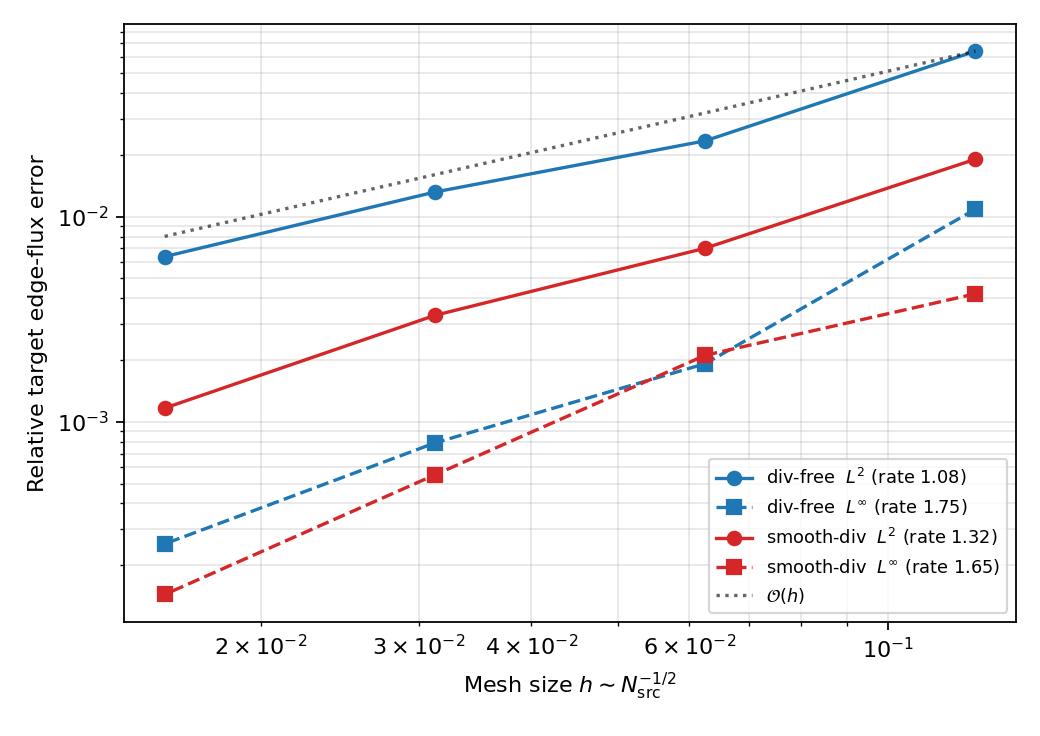
\includegraphics[width=\linewidth]{convergence.png}
\captionof{figure}{Edge-flux transfer convergence on Halton-Voronoi pairs, $N_s\!\in\!\{64,256,1024,4096\}$, $N_t\!\approx\!1.5\,N_s$. Both fields exhibit first-order $L^2$ convergence; $L^\infty$ rates are super-linear.}
\label{fig:conv}
\end{minipage}\hfill
\begin{minipage}{0.57\linewidth}\centering\small
\captionof{table}{Relative $L^2$ edge-flux error vs.\ $h$ for the two-stage remap.}
\label{tab:conv}
\vspace{2pt}
\begin{tabular}{lccccc}
\toprule
field        & $0.125$              & $0.0625$             & $0.0313$             & $0.0156$             & rate \\
\midrule
div-free     & $6.4\!\times\!10^{-2}$ & $2.3\!\times\!10^{-2}$ & $1.3\!\times\!10^{-2}$ & $6.4\!\times\!10^{-3}$ & \textbf{1.08} \\
smooth-div   & $1.9\!\times\!10^{-2}$ & $7.0\!\times\!10^{-3}$ & $3.3\!\times\!10^{-3}$ & $1.2\!\times\!10^{-3}$ & \textbf{1.32} \\
\bottomrule
\end{tabular}
\vspace{6pt}
\captionof{table}{Conservation residuals (smooth-div field, $N_s\!=\!256$, $N_t\!=\!384$). All four conservation properties hold at machine precision.}
\label{tab:cons}
\vspace{2pt}
\begin{tabular}{lc}
\toprule
quantity & max-abs residual \\
\midrule
global $\oint_{\partial\Omega}\uvec\!\cdot\!\nv\,ds$ (exact value $0$) & $\le 3\!\times\!10^{-15}$ \\
per source cell $|\!\sum\!\sigma_{K_s}(e)\Phi_e - d_s|K_s|\,|$       & $0$ (by construction) \\
per overlap $|\!\oint_{\partial(K_s\cap K_t)}\!\uh^{K_s}\!\cdot\!\nv\,ds - d_s|K_s\!\cap\!K_t|\,|$ & $5.7\!\times\!10^{-16}$ \\
per target cell $|\!\sum\!\sigma_{K_t}(e)\Phi_e - \sum_{K_s}\! d_s|K_s\!\cap\!K_t|\,|$ & $3.1\!\times\!10^{-17}$ \\
\bottomrule
\end{tabular}
\end{minipage}
\end{figure}

\paragraph{Convergence (Tab.~\ref{tab:conv}, Fig.~\ref{fig:conv}).}
Across $N_s\!\in\!\{64,\dots,4096\}$ both fields show first-order $L^2$ rate in the edge-flux error: 1.08 for the divergence-free field and 1.32 for the smooth-div field. The slightly super-linear rate on the second field reflects that the cell-mean divergence is captured exactly by the closed-form $d$ of~\eqref{eq:reconform}. $L^\infty$ rates are super-linear (1.76 and 1.66 respectively).

\paragraph{Projection visualisation (Fig.~\ref{fig:proj}).}
At $N_s\!=\!256$, $N_t\!=\!384$, the four panels per row show source fluxes (a), exact target fluxes (b), the transferred target fluxes (c) and the absolute error on each target edge (d), for both test fields. Computed and exact target fluxes are visually indistinguishable; the residual error on the divergence-free field is $\Vert e\Vert_\infty = 1.9\!\times\!10^{-3}$, on the smooth-div field $\Vert e\Vert_\infty = 2.1\!\times\!10^{-3}$. The error patterns concentrate where target edges nearly tangentially graze a source-cell boundary --- the geometric configuration the perpendicular tie-breaking probe is designed to handle robustly.

\begin{figure}[h]
\centering
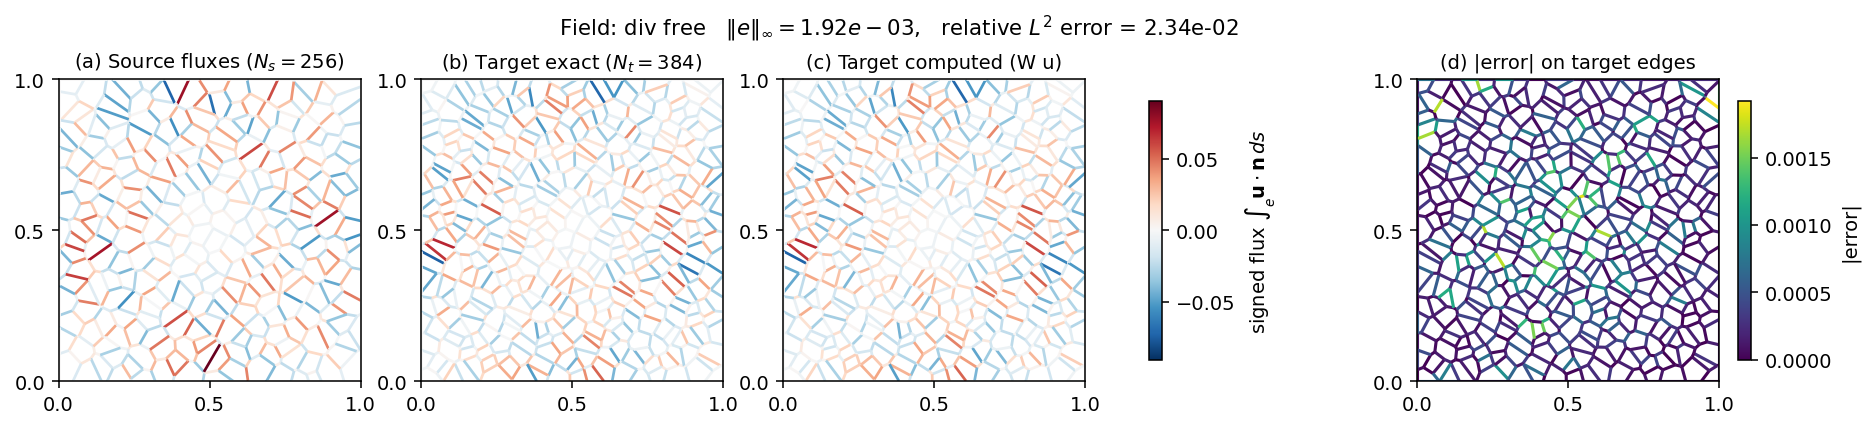
\includegraphics[width=\linewidth]{projection_div_free.png}\\[1pt]
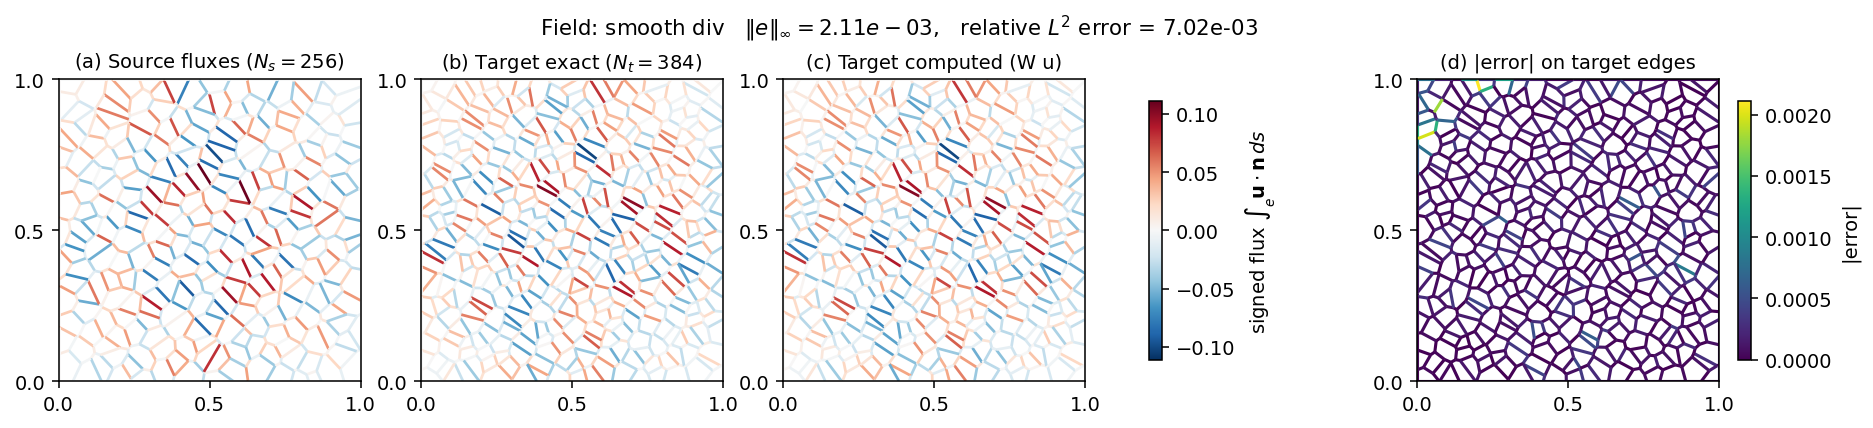
\includegraphics[width=\linewidth]{projection_smooth_div.png}
\caption{Top row: divergence-free field $\uvec^{\mathrm{df}}$. Bottom row: smooth-divergence field $\uvec^{\mathrm{sd}}$. $N_s\!=\!256$, $N_t\!=\!384$. Each panel: (a) source edge fluxes; (b) exact target fluxes; (c) transferred target fluxes (after Stage 2); (d) absolute error on each target edge.}
\label{fig:proj}
\end{figure}

\paragraph{Conservation across scales (Tab.~\ref{tab:cons}).}
Four layers are reported: \emph{global} (boundary integral matches exact $0$ to $10^{-15}$), \emph{per source cell} (trivially exact by~\eqref{eq:discdiv}), \emph{per overlap} ($\le 5.7\!\times\!10^{-16}$ across $174$ sampled $(K_s,K_t)$ overlaps), and \emph{per target cell} ($3.1\!\times\!10^{-17}$, satisfied at machine precision because the constraint \eqref{eq:hdiv-constraint} is enforced by Stage 2).

\paragraph{Per-cell divergence convergence (Fig.~\ref{fig:divconv}).}
We sweep the per-cell divergence error in the area-weighted relative $L^2$ norm
$e_{\mathrm{div}}^2 = \sum_K |K|(d_K^{\text{disc}} - d_K^{\text{exact}})^2 / \sum_K |K|(d_K^{\text{exact}})^2$
on the smooth-div field, plotted on separate panels for source and target so the machine-precision source curve does not skew the target axis. \emph{Source} (left): the discrete divergence theorem~\eqref{eq:discdiv} acting on edge fluxes integrated to machine precision keeps the residual at $10^{-9}$--$10^{-15}$ at every refinement; the descending floor reflects the shrinking analytic-side quadrature error on smaller cells. \emph{Target} (right): the H(div)-projected fluxes give a target divergence error decaying from $4.3\!\times\!10^{-2}$ at $h\!=\!0.125$ to $4.8\!\times\!10^{-3}$ at $h\!=\!0.0156$, fitted slope $\mathbf{1.04}$.

\begin{figure}[!htb]
\centering
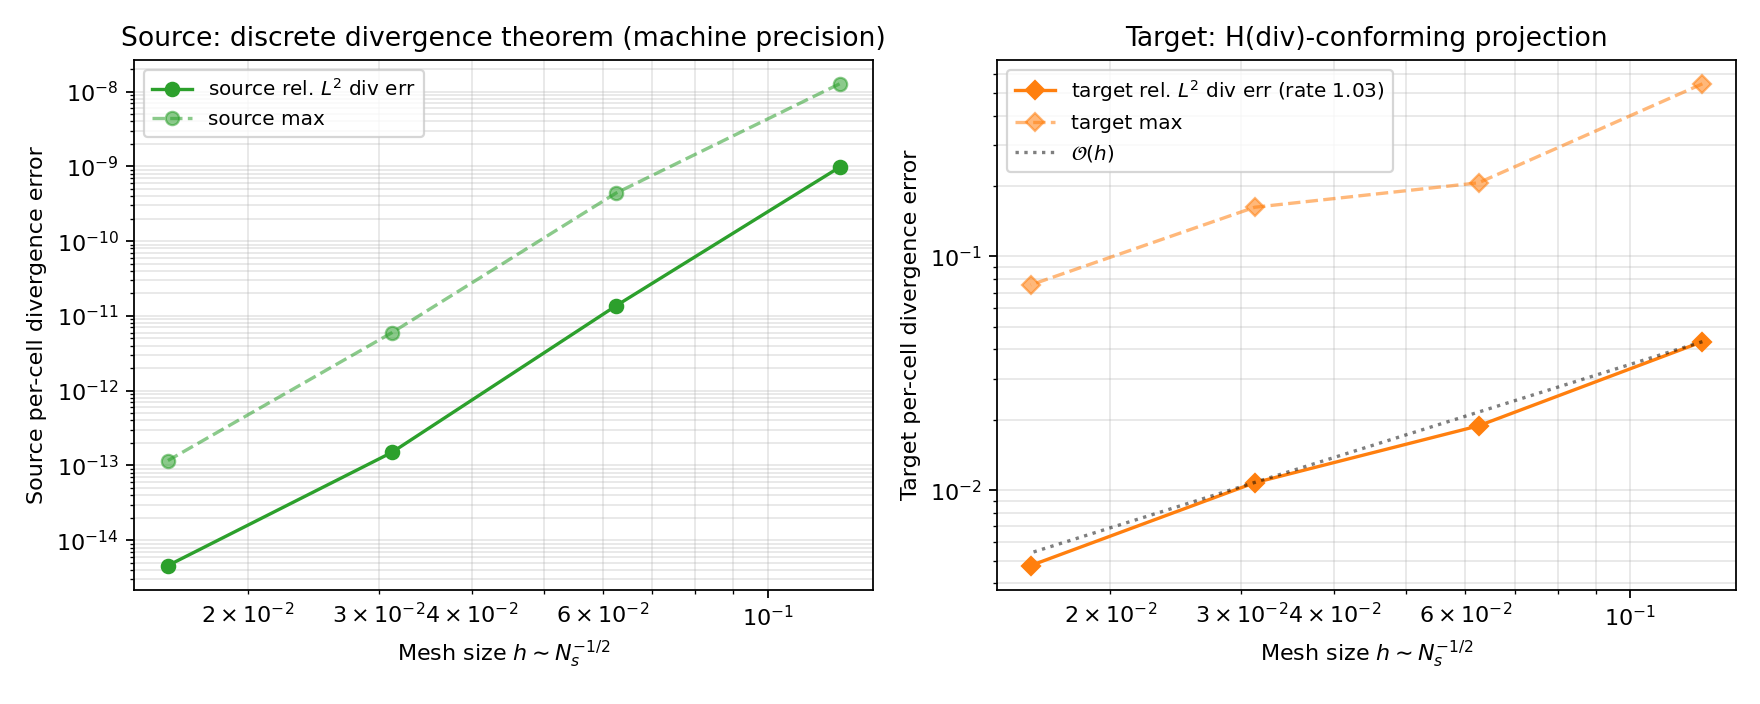
\includegraphics[width=0.78\linewidth]{divergence_convergence.png}
\caption{Per-cell divergence error vs.\ $h$, smooth-div field. \emph{Left:} source mesh stays at machine precision (floor $10^{-9}$--$10^{-15}$, set by the analytic-side quadrature). \emph{Right:} target mesh after the H(div)-conforming projection of~\eqref{eq:hdiv-constraint}; the relative $L^2$ divergence error converges as $\mathcal{O}(h)$ with rate $\mathbf{1.04}$.}
\label{fig:divconv}
\end{figure}

Weights are written in SCRIP \cite{Jones1999} with each edge as a ``cell'' (center = midpoint, corners = endpoints, area = edge length); the matrix is 1-based source/destination address arrays and a scalar weight per link.

%==========================================================
\section{Conclusion}
%==========================================================

The two-stage first-order mimetic edge-flux remap is exactly conservative on every source-target overlap and at the global integral level, satisfies the per-target-cell discrete-divergence constraint at machine precision, and converges at first order in the $L^2$ norm of edge fluxes for smooth analytical fields including divergence-free fields. Per-cell divergence is exact on the source mesh and converges at first order on the target mesh. The output is a single signed scalar per unique edge in the intrinsic-normal convention.

\enlargethispage{4\baselineskip}
\begin{multicols}{2}
{\scriptsize
\bibliographystyle{plain}
\bibliography{references}
}
\end{multicols}

\end{document}
